\chapter{Survival analysis}
\section{Survivor functions for whole sample}
In the fourth exercise we do survival analysis with data from lung cancer patients. The three variables used here are \texttt{PRE30}, indicating whether the patient is a smoker, \texttt{AGE}, encoding the age at surgery, and \texttt{Risk1Y}, indicating whether the patient died within one year after the surgery. The first observations are shown in Table \ref{5table}. Hence, this data can be understood as interval censored survival data. In this exercise we were asked to assume failure times at \texttt{AGE}+1, if the patient died and fit survivor functions to model $S(t)=P(T>t)$, where $T$ is a random variable encoding the failure time of an object, here the time of death of a patient. 
\begin{table}[ht]
\centering
\begin{tabular}{llrl}
  \hline
 & PRE30 & AGE & Risk1Y \\ 
  \hline
1 & TRUE &  60 & FALSE \\ 
  2 & TRUE &  51 & FALSE \\ 
  3 & TRUE &  59 & FALSE \\ 
  4 & FALSE &  54 & FALSE \\ 
  5 & TRUE &  73 & TRUE \\ 
  6 & FALSE &  51 & FALSE \\ 
   \hline
\end{tabular}
\caption{First observations of the lung cancer patient data set.}
\label{5table}
\end{table}

To assess which parametric model is reasonable for the data, we use non-parametric estimators for the survival curve. Therefore we draw the Kaplan-Meier estimator, given by $$\hat{S}_{KM}(t)=\prod_{\{j:\tau_j<t\}}(1-\frac{d_j}{r_j}),$$ where $0\leq \tau_1<\tau_2<...$ denote the ordered uncensored failure times (here \texttt{AGE}+1), $r_i$ and $d_i$ the number of units still at risk and failures at $\tau_i$ respectively. A similar estimator, especially in those areas where still many cases are at risk, is the Fleming-Harrington estimator $$\hat{S}_{FH}(t)=\prod_{\{j:\tau_j<t\}}\exp(-\frac{d_j}{r_j}).$$ Both are shown in Figure \ref{5nonpar} where we can see that they only differ obviously at ages $>80$. In the area of lower risk both seem to be identical, why we can't see the orange line. We can also see that the confidence band spreads as the survival probability decreases. Both curves are fitted using \texttt{survfit} from the package \textit{survival} which also computes pointwise confidence intervals using Greenwood's formula.  
\begin{figure}[!t]
\centering
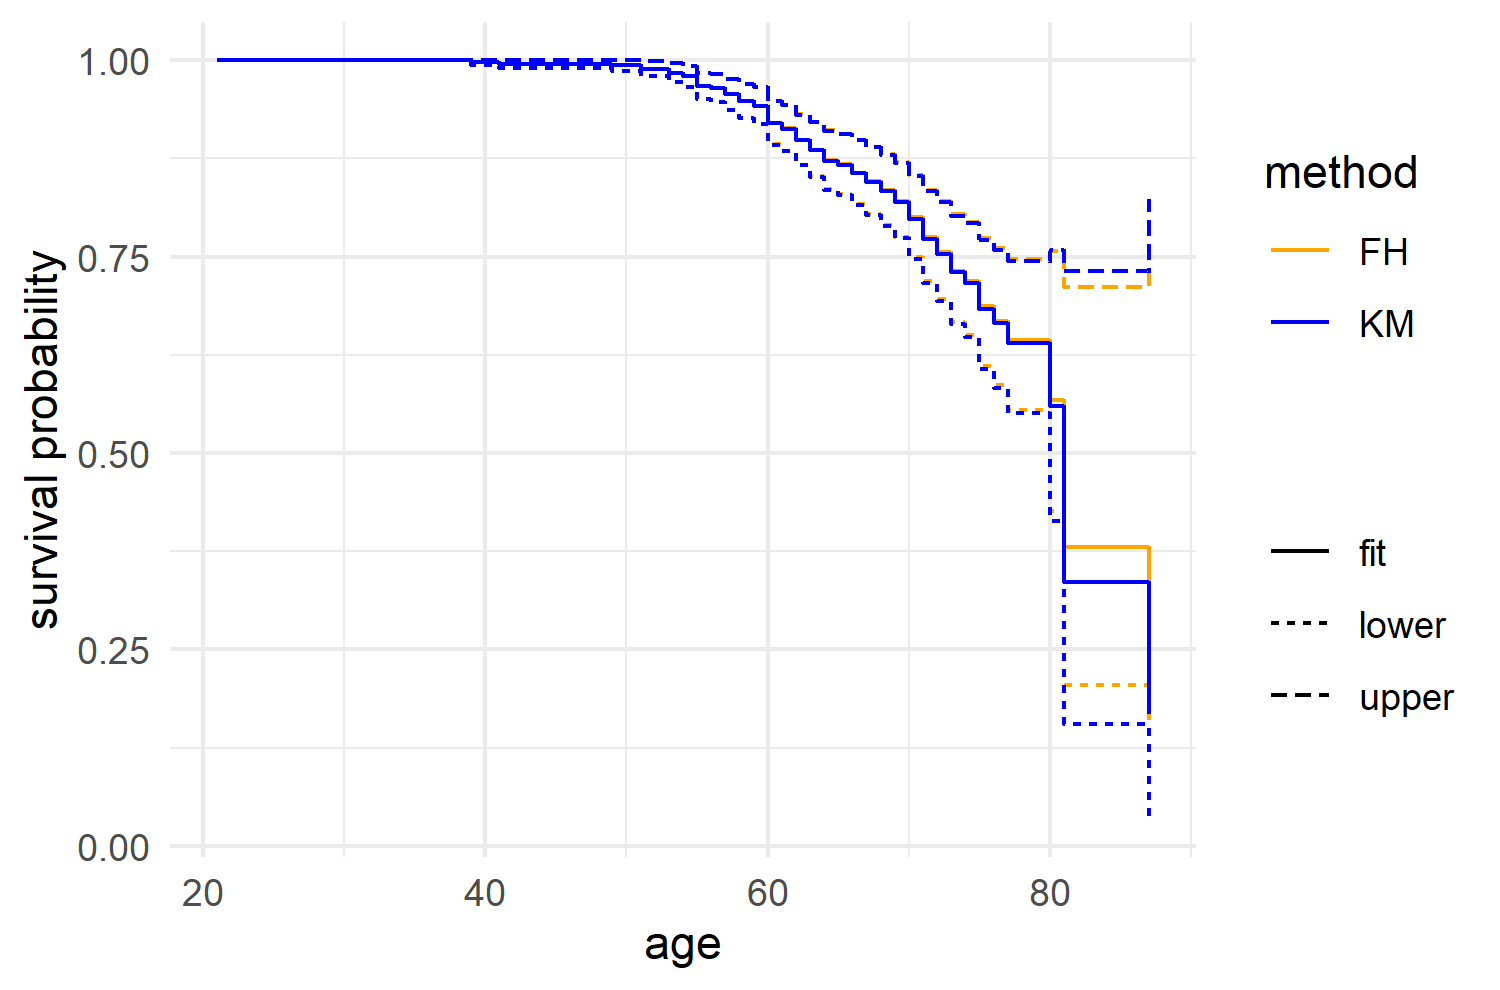
\includegraphics[width=0.7\textwidth, keepaspectratio]{ex4/survfits.png}
\caption{Nonparametric estimators for the survivor function. KM = Kaplan-Meier drawn in blue; FH=Fleming-Harrington in orange. Dashed lines show the confidence bands.}
\label{5nonpar}
\end{figure}
\begin{figure}[!b]
\centering
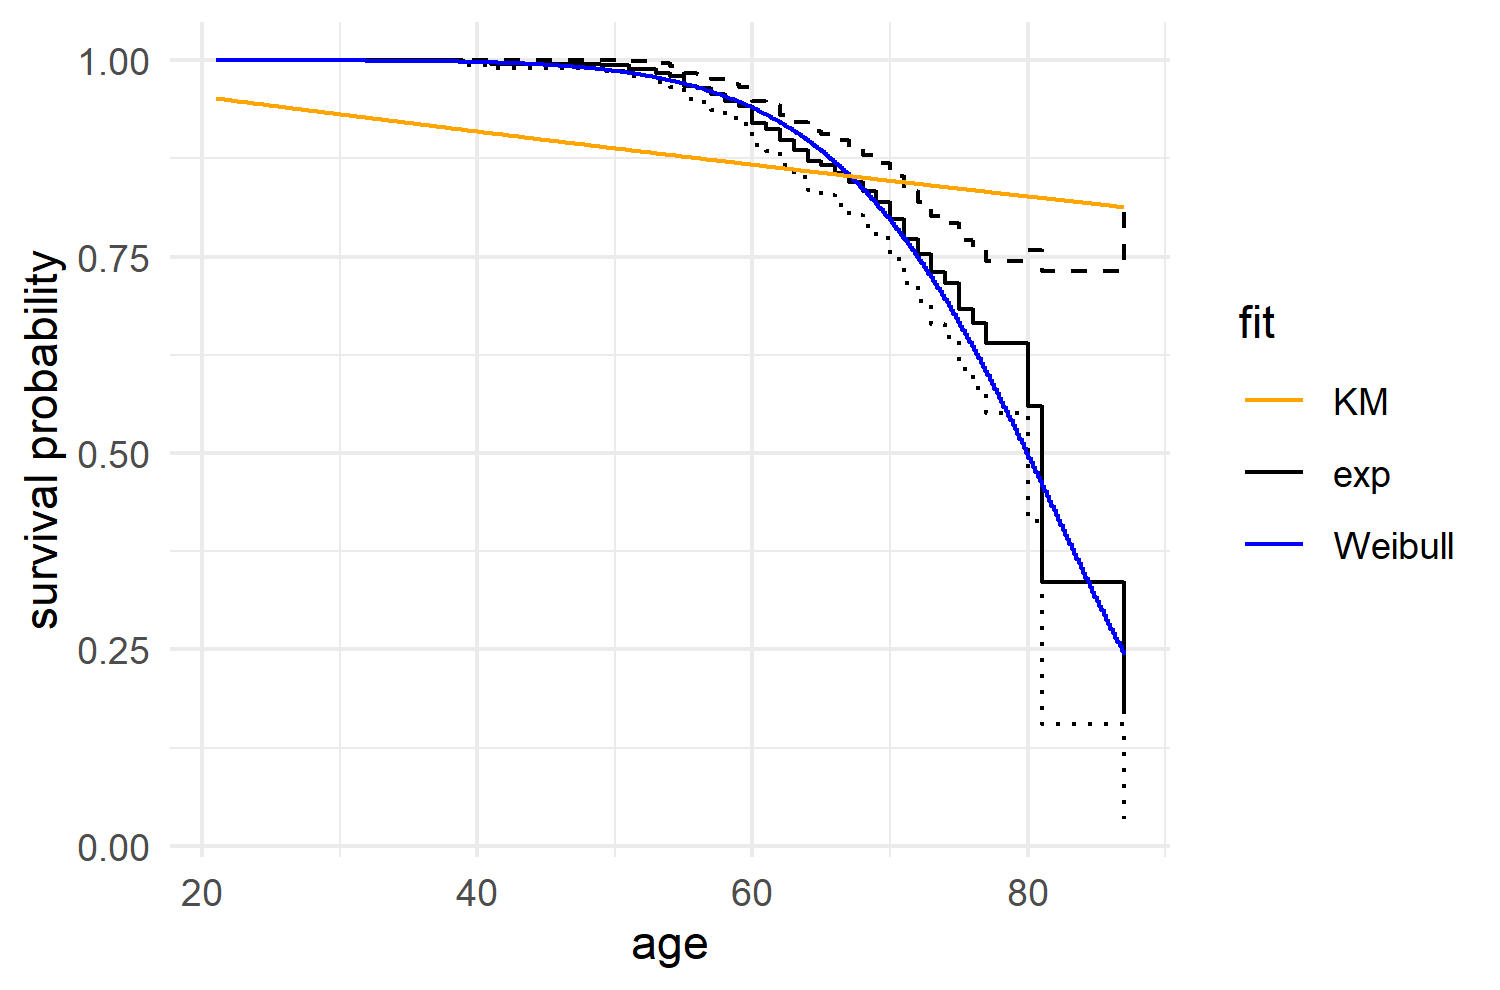
\includegraphics[width=0.7\textwidth, keepaspectratio]{ex4/paramsurvfits.png}
\caption{KM estimator and parametric fits for the survivor function. Dashed lines represent the confidence band of the KM estimator. Exponential fit in orange; Weibull fit in blue.}
\label{5parfit}
\end{figure}

With the function \texttt{survreg} we can fit parametric models to the data. Typical models are the exponential, Weibull and log-logistic models. Because we were asked to fit the first two in this exercise, I only give more details on them. The exponential model assumes a constant Hazard function, i.e. rate of failure, of $\lambda$ over time resulting in an exponential survivor function $S_{exp}(t)=\exp(-\lambda t)$. With the Weibull distribution we can handle varying Hazard rates by taking $h(t)=\alpha \lambda ^{\alpha} t^{\alpha-1}$ resulting in a survivor function $S(t)=\exp(-(\lambda t)^\alpha)$. At $t=1$ we have $h(1)=\alpha\lambda^\alpha$, so $\lambda$ is still the parameter of failure rate, defined for the unit time and modified by the shape parameter. Obviously we get the exponential model for $\alpha=1$, an increasing Hazard function for $\alpha>1$ and an decreasing Hazard or $0<\alpha<1$. The Weibull distribution is often more appropriate when we can't assume constant Hazard rates. In clinical studies concerning relapses of psychological diseases for example a relapse, i.e. failure, gets often less probable with time since recovery. Here a decreasing Hazard function would be appropriate. But in general older living organisms have a smaller survivor probability over time than younger ones indicating the use of an increasing Hazard. In this example the fits (see Figure \ref{5parfit}) compared to the nonparametric KM estimator suggest that an exponential model can be rejected quite obviously, since the shape does not at all represent the step function. The Weibull model on the other hand seems very good as it follows the KM estimation pretty directly. Although it lies beneath the lower confidence bound at an age around 78, the overall shape suits pretty well.  

\section{Comparison of smokers and non-smokers}
Now we split the data set into two parts - smokers and non-smokers - according to the variable \texttt{PRE30}. Fitting a KM estimate for each group leads to Figure \ref{5nonpargroups}. We see very clear that the curve of smokers is stepper than the other. The curve for nonsmokers drops in the end since the only patient with age 81 in the nonsmokers group, who also was the oldest one, died. But all in all the survival probability of nonsmokers seems higher. In the plot we also see that there are more steps in the curve for the smokers. This is because of the unbalanced sample sizes. With 386 smokers and 84 nonsmokers the proportion of smokers is 82.12$\%$. It is well known that smoking increases the probability to get cancer, so this is not a surprising observation here. An inferential comparison of the two groups to check whether the visual differences are statistically significant is done with a log-rank test. With the R function \texttt{survdiff} in the same package we get the results $\chi ^2=2.7$ and $p=.1$. This indicates a difference between the groups, too, which most researchers won't interpret as significant. Since I am no expert in this area, I can't finally judge it, but would emphasize that the difference may be statistically relevant in this case.
\begin{figure}[!htb]
\centering
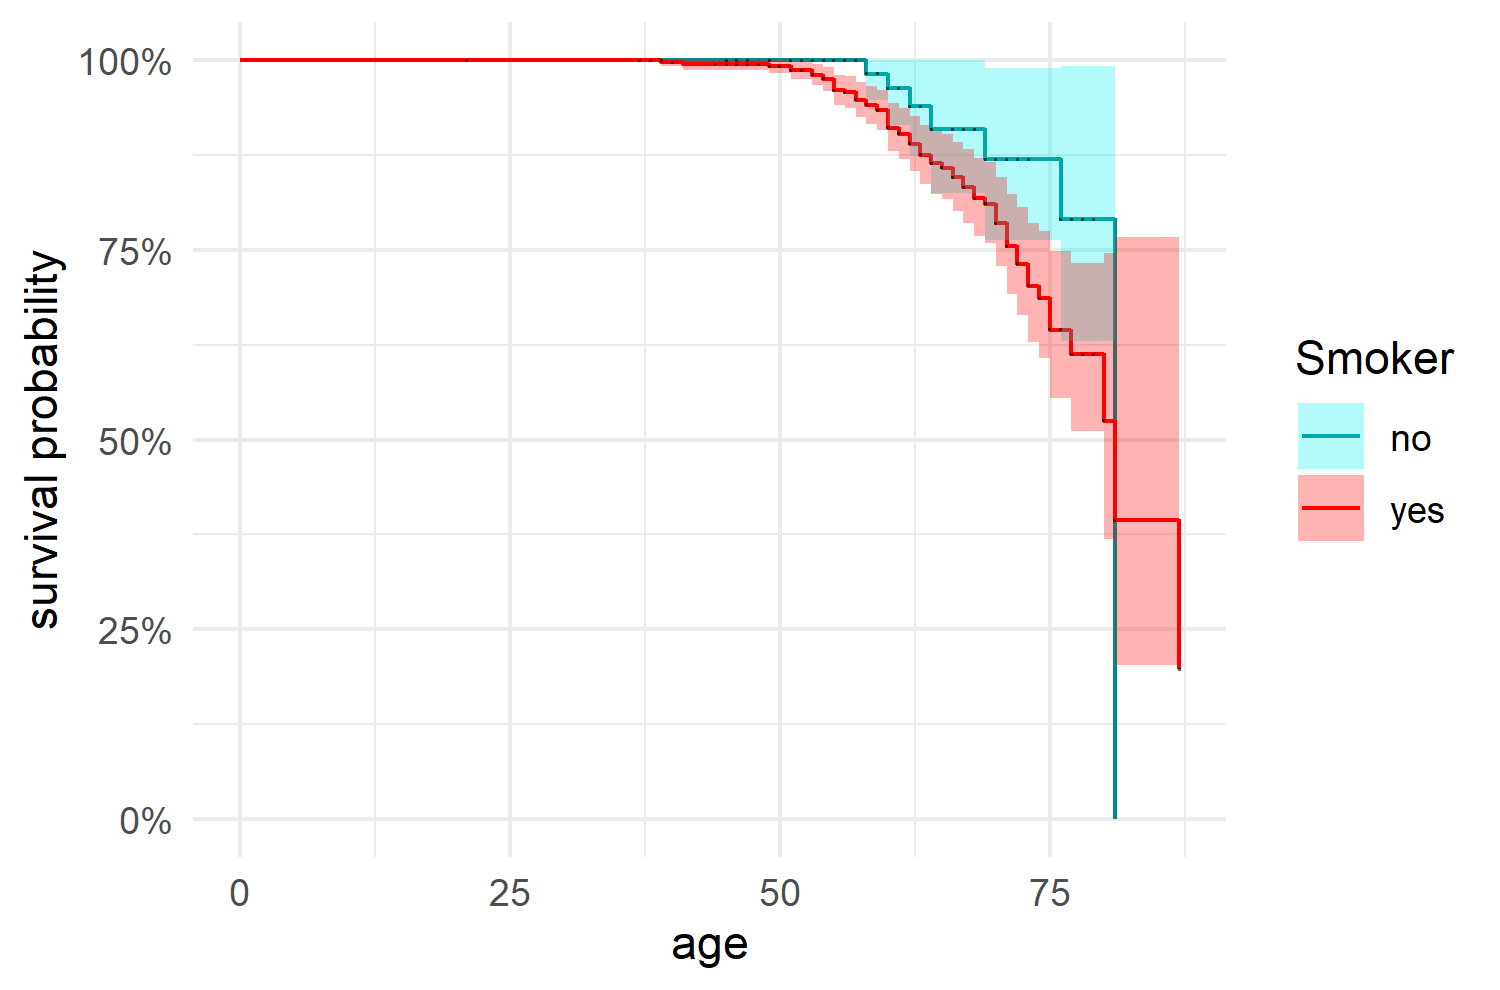
\includegraphics[width=0.8\textwidth, keepaspectratio]{ex4/smokers.png}
\caption{Kaplan-Meier estimate for smokers (red) and nonsmokers (blue) with confidence bands.}
\label{5nonpargroups}
\end{figure} 

Now we want to check whether the assumption of a Weibull model is still justified when we look at the groups separately. Therefore we fitted a Weibull curve for each of the groups (see Figure \ref{5paragroups}). For the group of smokers we see like above a very good fit. For nonsmokers the Weibull fit looks quite well but is probably distorted by the sudden drop down in the end. It seems like a less steep curve would fit better to the data in the beginning. This may be solved by an extended sample where especially more older patient are included. Of course, this is sometimes hard to accomplish in practice. Still the Weibull curve of the smokers group decreases faster than the other and I would finally conclude, also because it seems quite reasonable (although a statistician should argue rather with data than with common sense), that smoking decreases the probability of surviving one year after the surgery. 
\begin{figure}[!h]
\centering
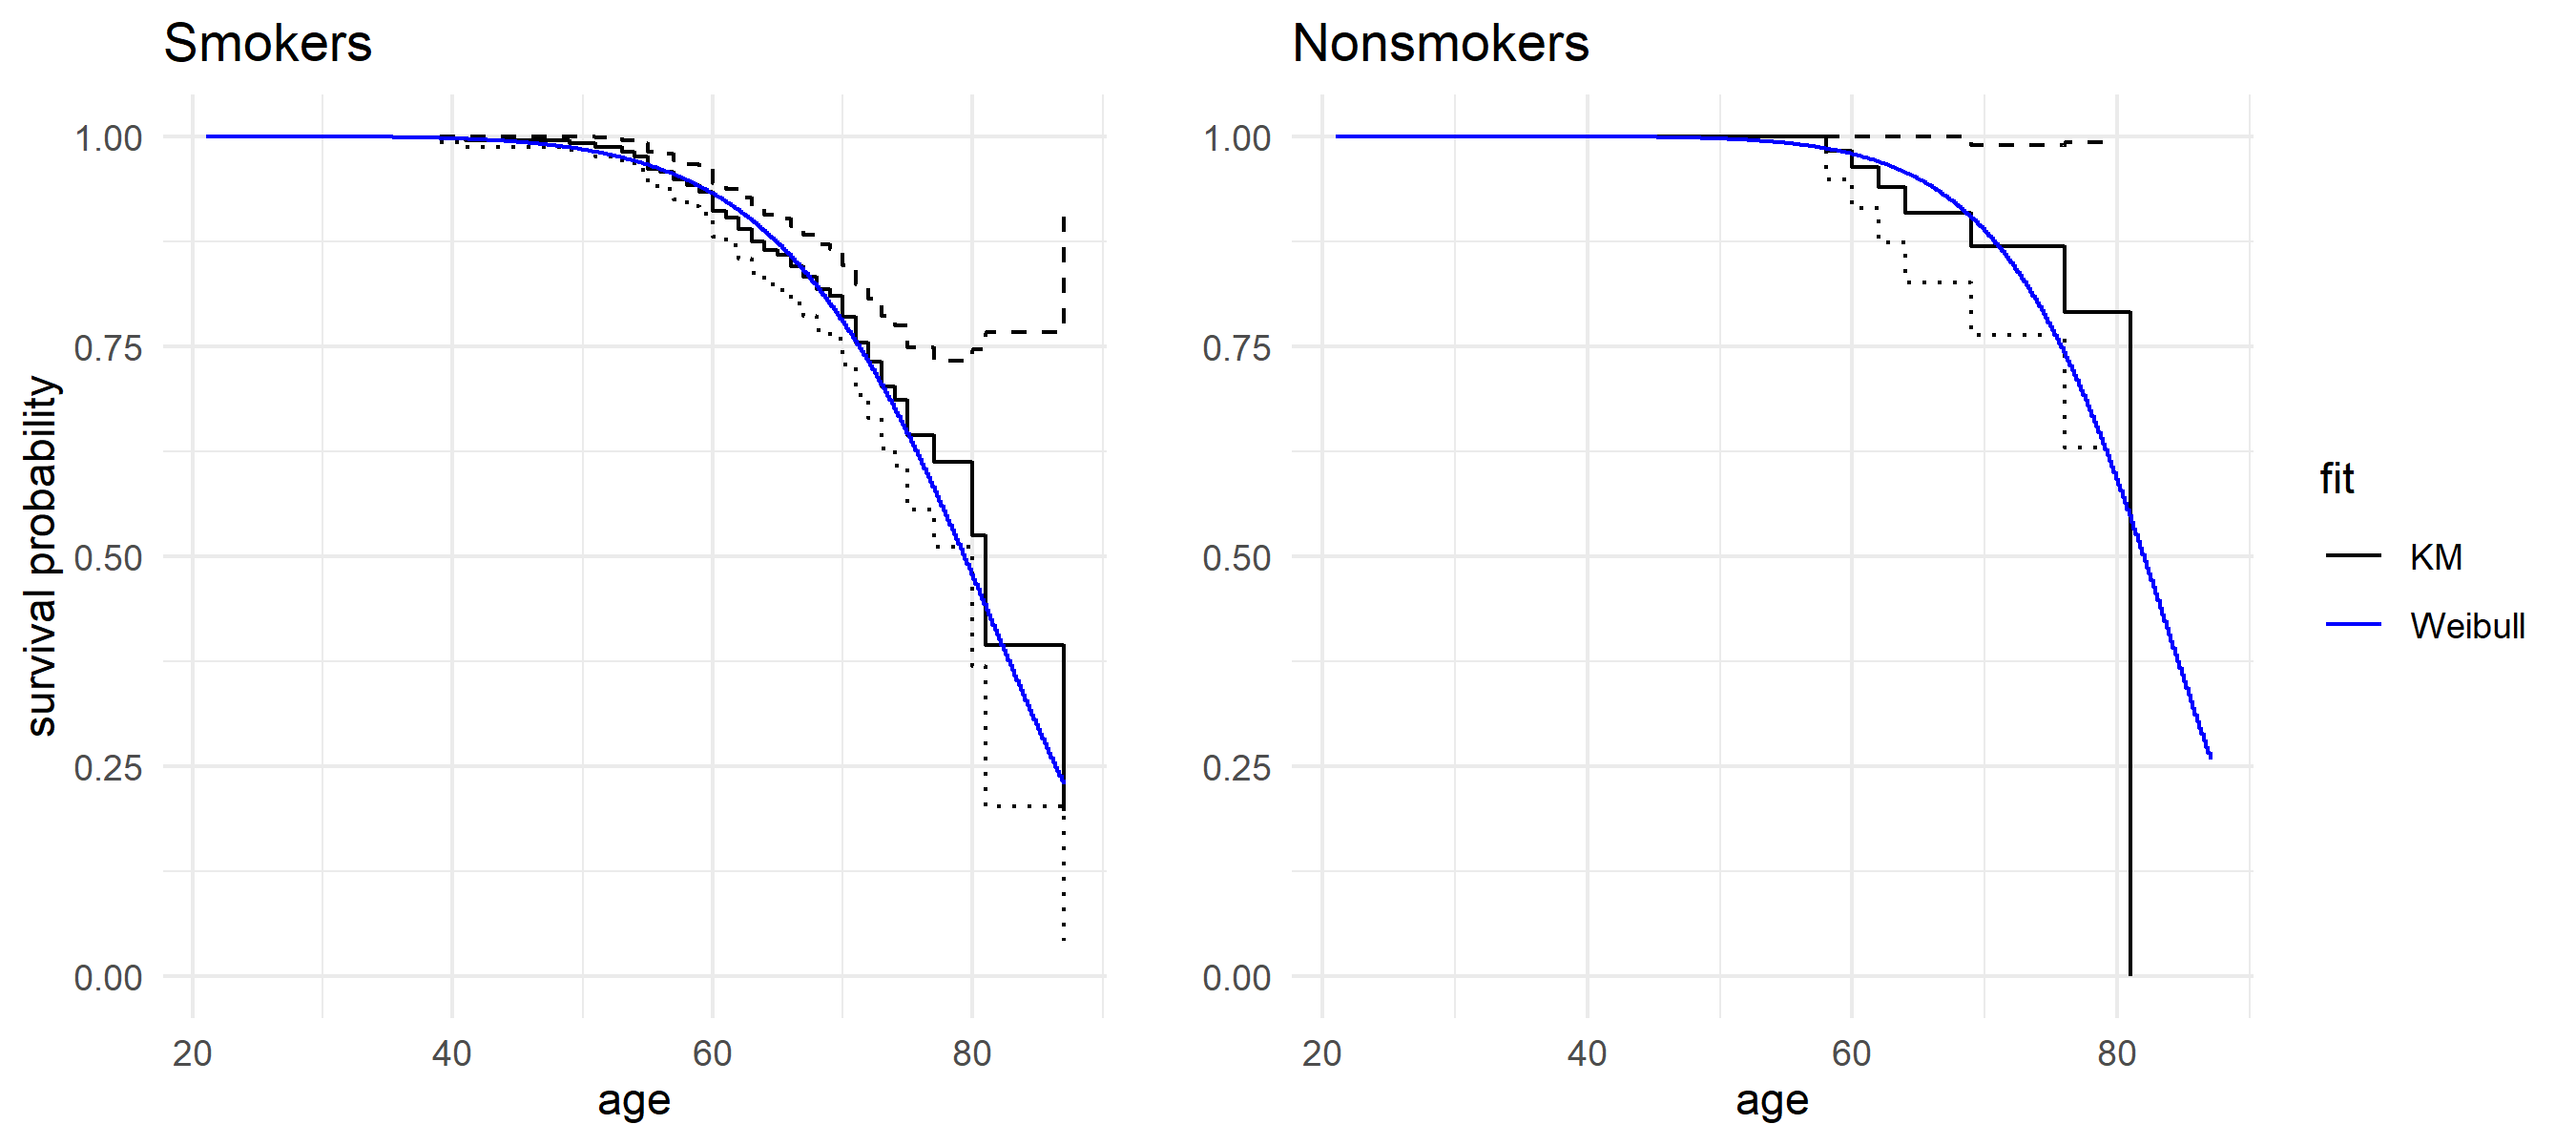
\includegraphics[width=\textwidth, keepaspectratio]{ex4/groupsparam}
\caption{Kaplan-Meier estimate with dashed confidence bands (black) and Weibull fit (blue) for patient groups of smokers (left) and nonsmokers (right).}
\label{5paragroups}
\end{figure}